\documentclass[12pt, oneside, titlepage]{article}   	% use "amsart" instead of "article" for AMSLaTeX format
\usepackage{geometry}                     
\usepackage{amsmath}                      
\usepackage{amssymb}                       
\usepackage{bm}   
\usepackage{tabularx}   
\usepackage{caption}          
 \captionsetup[table]{labelfont=sc}

\usepackage{booktabs}

\usepackage{graphicx}


%%%%%%%%%%%%%%%%%%%%%%%%%%%%%%%%%%%%%%%%%%%%%%%%%%%%
%%%%%%%%%%%%%%%%%%%%%%%%%%%%%%%%%%%%%%%%%%%%%%%%%%%%
% begin document
%%%%%%%%%%%%%%%%%%%%%%%%%%%%%%%%%%%%%%%%%%%%%%%%%%%%
%%%%%%%%%%%%%%%%%%%%%%%%%%%%%%%%%%%%%%%%%%%%%%%%%%%%

\begin{document}

\begin{center}
\captionof{table}{ Summary of data sets used to estimate parameters. } \label{tab:title1} 
 \begin{tabularx}{\linewidth}{ l l c c } 
 \hline
 \hline
\multicolumn{1}{ c }{ Parameter data } & 
\multicolumn{1}{ c }{ Description } & 
\multicolumn{1}{ c }{ Data set }  & 
\multicolumn{1}{ c }{ Time span } \\
 \hline
 % seed bag burial experiment
 \textsc{Seed vital rates} & --- & --- & --- \\ 
 Seed survival and germination & Seed bag burial & $\bm{\mathrm{Y}}_1$ & 2006-2009  \\ 
 Seed viability & Viability trials & $\bm{\mathrm{Y}}_2$ & 2006-2009 \\ 
 Seed survival and germination & Seed pots & $\bm{\mathrm{Y}}_3$ & 2013-2019  \\ 
 \textsc{Seedling survival} & --- & --- & --- \\ 
 Seedling survival to fruiting & Field surveys & $\bm{\mathrm{Y}}_4$ & 2006-2019 \\ 
 \textsc{Fruits per plant} & --- & --- & --- \\ 
 Total fruit equivalents per plant & Field surveys & $\bm{\mathrm{Y}}_5$ & 2006-2012 \\ 
 Undamaged and damaged fruits per plant & Field surveys & $\bm{\mathrm{Y}}_6$ & 2013-2019 \\ 
 \textsc{Seeds per fruit} & --- & --- & --- \\ 
  Seeds per undamaged fruit & Lab counts & $\bm{\mathrm{Y}}_7$ & 2006-2019 \\ 
  Seeds per damaged fruit & Lab counts & $\bm{\mathrm{Y}}_8$ & 2013-2019 \\   
  \hline
\end{tabularx}
\end{center}

\newpage

\begin{center}
\captionof{table}{ Description of key parameters. } \label{tab:title2} 
 \begin{tabularx}{\linewidth}{c X} 
 \hline
 \hline
\multicolumn{1}{ c }{ Parameter } & 
\multicolumn{1}{ c }{ Description } \\
 \hline
 % seed bag burial experiment
 $\theta_1$ & Probability of survival of seeds from October in year $t$ to January in year $t+1$, for seeds produced in year $t$ \\ 

 $\theta_2$ & Probability of emergence of seeds in January in year $t+1$, conditional on being intact or a germinant in January in year $t+1$, for seeds produced in year $t$ \\
 
 $\theta_3$ & Probability of survival of seeds from January in year $t+1$ to October in year $t+1$, conditional on being intact in January in year $t+1$, for seeds produced in year $t$  \\
 
 $\theta_4$ & Probability of survival of seeds from October in year $t$ to January in year $t+2$, for seeds produced in year $t$ \\
  
 $\theta_5$ & Probability of emergence of seeds in January in year $t+2$, conditional on being intact or a germinant in January in year $t+2$, for seeds produced in year $t$  \\
 
 $\nu_1$ & Probability of viability for seeds in October of year $t+1$, for seeds produced in year $t$ \\
 
 $\nu_2$ & Probability of survival for seeds in October of year $t+2$, for seeds produced in year $t$ \\

 $\sigma$ & Probability of survival of seedlings to fruiting plants\\

 $F$ & Number of fruits per plant \\
 
 $\phi$ & Number of seeds per undamaged fruit \\ 
  \hline
\end{tabularx}
\end{center}

\newpage

% header for seed burial data table

%\begin{table}[ht]
%\centering
%\begin{tabular}{lcccccc}
%  \hline
%  \hline
% &  \multicolumn{3}{c}{Age 1} & \multicolumn{2}{c}{Age 2} & Age 3 \\
% \cmidrule(lr){2-4} \cmidrule(lr){5-6} \cmidrule(lr){7-7} 
%Population & 2007 & 2008 & 2009 & 2008 & 2009 & 2009 \\ 
%  \hline

%%%%%%%%%%%%%%%%%%%%%%%%%%%%%%%%%%
% SEED BAG BURIAL EXPERIMENT
%%%%%%%%%%%%%%%%%%%%%%%%%%%%%%%%%%

% latex table generated in R 3.6.2 by xtable 1.8-4 package
% Tue Mar 24 16:48:39 2020
\captionof{table}{ Summary of dataset from seed bag burial experiment. [Data set $\bm{\mathrm{Y}}_1$]  } \label{tab:titleburial} 
\begin{table}[ht]
\centering
\begin{tabular}{lcccccc}
  \hline
  \hline
 &  \multicolumn{3}{c}{Age 1} & \multicolumn{2}{c}{Age 2} & Age 3 \\
 \cmidrule(lr){2-4} \cmidrule(lr){5-6} \cmidrule(lr){7-7} 
Population & 2007 & 2008 & 2009 & 2008 & 2009 & 2009 \\ 
  \hline
BG &   7 &  10 &  10 &   6 &  10 &   3 \\ 
  BR &  10 &  10 &  10 &   9 &  10 &   9 \\ 
  CF &  10 &  10 &  10 &  10 &  10 &  10 \\ 
  CP3 &   7 &  10 &   8 &   9 &   5 &   7 \\ 
  DEM &   8 &   9 &  10 &   7 &   7 &   6 \\ 
  DLW &   9 &   9 &   8 &   8 &   9 &   6 \\ 
  EC &   9 &   9 &  10 &   8 &  10 &   8 \\ 
  FR &   9 &   7 &  10 &   8 &   9 &   3 \\ 
  GCN &  10 &  10 &  10 &   9 &   9 &   6 \\ 
  KYE &  10 &  10 &  10 &   9 &   9 &   9 \\ 
  LCE &  10 &  10 &   9 &   9 &   7 &   7 \\ 
  LCW &  10 &  10 &   5 &   9 &   7 &   8 \\ 
  LO &  10 &   9 &  10 &  10 &  11 &   9 \\ 
  MC &  10 &  10 &  10 &   8 &   9 &   9 \\ 
  OKRE &  10 &  11 &  10 &   9 &   7 &   9 \\ 
  OKRW &  10 &  10 &   8 &   9 &   9 &   7 \\ 
  OSR &  10 &  10 &  10 &   8 &   9 &   9 \\ 
  S22 &   9 &  10 &  10 &   8 &  10 &   8 \\ 
  SM &   9 &  10 &   9 &   8 &  10 &   9 \\ 
  URS &   7 &   9 &   9 &   5 &   9 &   3 \\ 
   \hline
\end{tabular}
\end{table}
 
 \newpage
 
%%%%%%%%%%%%%%%%%%%%%%%%%%%%%%%%%%
% VIABILITY FOR SEED BAG BURIAL EXPERIMENT
%%%%%%%%%%%%%%%%%%%%%%%%%%%%%%%%%%

% latex table generated in R 3.6.2 by xtable 1.8-4 package
% Tue Mar 24 17:14:38 2020
\captionof{table}{ Summary of dataset on viability of seeds from seed bag burial experiment. [Data set $\bm{\mathrm{Y}}_2$] } \label{tab:titleviab} 
\begin{table}[ht]
\centering
\begin{tabular}{lcccccc}
  \hline
  \hline
 &  \multicolumn{3}{c}{Age 1} & \multicolumn{2}{c}{Age 2} & Age 3 \\
 \cmidrule(lr){2-4} \cmidrule(lr){5-6} \cmidrule(lr){7-7} 
Population & 2007 & 2008 & 2009 & 2008 & 2009 & 2009 \\ 
  \hline
BG &   7 &  10 &  10 &   6 &  10 &   3 \\ 
  BR &  10 &   9 &  10 &  10 &  10 &   9 \\ 
  CF &  10 &  10 &  10 &   9 &  10 &  10 \\ 
  CP3 &   7 &  10 &   9 &   8 &   7 &   7 \\ 
  DEM &   8 &   9 &  10 &   6 &   7 &   5 \\ 
  DLW &   8 &   9 &   9 &   8 &   9 &   7 \\ 
  EC &   9 &  10 &  10 &   8 &  10 &   6 \\ 
  FR &   8 &   8 &  10 &   8 &  10 &   4 \\ 
  GCN &   9 &  10 &  10 &   8 &   9 &   7 \\ 
  KYE &  10 &  10 &  10 &   9 &   9 &   9 \\ 
  LCE &  10 &  10 &   9 &   9 &   6 &   9 \\ 
  LCW &  10 &  10 &   5 &   9 &   7 &   7 \\ 
  LO &  11 &   9 &  10 &   9 &  10 &   9 \\ 
  MC &   9 &   9 &  10 &   8 &   9 &   9 \\ 
  OKRE &  10 &  11 &  10 &   9 &   7 &   9 \\ 
  OKRW &   9 &  10 &   8 &   8 &   9 &   7 \\ 
  OSR &  10 &  10 &  10 &   8 &   9 &   9 \\ 
  S22 &   9 &  10 &  10 &   8 &  10 &   8 \\ 
  SM &   8 &  10 &   9 &   8 &  10 &  11 \\ 
  URS &   7 &   9 &   9 &   5 &   8 &   4 \\ 
   \hline
\end{tabular}
\end{table}

 \newpage
 
%%%%%%%%%%%%%%%%%%%%%%%%%%%%%%%%%%
% SEEDLING SURVIVAL TO FRUITING
%%%%%%%%%%%%%%%%%%%%%%%%%%%%%%%%%%

% latex table generated in R 3.6.2 by xtable 1.8-4 package
% Wed Mar 25 10:25:29 2020
\captionof{table}{ Summary of dataset on seedling survival to fruiting. [Data set $\bm{\mathrm{Y}}_4$] } \label{tab:sigma} 
\begin{table}[ht]
\centering
\begin{tabular}{lcccccccccc}
  \hline
Population & 2006 & 2007 & 2008 & 2009 & 2010 & 2011 & 2012 & 2013 & 2014 & 2015 \\ 
  \hline
BG &  18 &  21 &  22 &  26 &  24 &  26 &  20 &  23 &   3 &  26 \\ 
  BR &  19 &  30 &  29 &  30 &  30 &  30 &  29 &  30 &   9 &  27 \\ 
  CF &  20 &  21 &  28 &  29 &  29 &  21 &  23 &  27 &  15 &  15 \\ 
  CP3 &  18 &  19 &  19 &  13 &  19 &   8 & NA &  10 &   1 &   7 \\ 
  DEM &  18 &  17 &  14 &  21 &  24 &  25 &  18 &  22 &   3 &   9 \\ 
  DLW &  16 &  18 &  13 &  15 &  17 &  22 &  16 &  19 &   1 &  13 \\ 
  EC &  20 &  28 &  30 &  30 &  30 &  30 &  30 &  24 &   2 &  10 \\ 
  FR &  20 &  28 &  27 &  27 &  30 &  30 &  24 &  25 &   7 &  15 \\ 
  GCN &  18 &  20 &  15 &  20 &  28 &  29 &  22 &  27 &   5 &  17 \\ 
  KYE &  18 &  28 &  28 &  30 &  29 &  30 &  27 &  28 &   1 &  27 \\ 
  LCE &  20 &  12 &  18 &  19 &  19 &   1 &   1 &   3 &   1 &   8 \\ 
  LCW &  16 &  27 &  27 &  27 &  21 &   4 & NA &  15 & NA &   1 \\ 
  LO &  12 &  15 &  28 &  29 &  27 &   2 &   1 &  19 &   5 &  11 \\ 
  MC &  17 &  11 &  22 &  25 &  27 &  30 &  29 &  27 &   6 &  18 \\ 
  OKRE &  14 &  10 &   8 &  19 &  21 &  17 &   7 &  19 &   6 &  10 \\ 
  OKRW &  19 &  19 &  22 &  20 &  19 &  12 &   9 &  13 & NA &   3 \\ 
  OSR &  15 &  13 &   9 &   9 &  23 &  26 &  18 &  20 &   1 &  14 \\ 
  S22 &  17 &  10 &  21 &  18 &  28 &  17 &  27 &  26 & NA &  17 \\ 
  SM &  15 &   8 &  13 &  18 &  23 &  25 &  18 &  24 & NA &  19 \\ 
  URS &   4 &  17 &  10 &   7 &  12 &  14 &   3 &   5 &   2 &   1 \\ 
   \hline
\end{tabular}
\end{table}

The data 
 
 \newpage
 
 % latex table generated in R 3.6.2 by xtable 1.8-4 package
% Wed Mar 25 10:41:34 2020
 \captionof{table}{ Summary of undercounting in the dataset on seedling survival to fruiting. } \label{tab:undercount} 
\begin{table}[ht]
\centering
\begin{tabular}{lcccccccccc}
  \hline
site & 2006 & 2007 & 2008 & 2009 & 2010 & 2011 & 2012 & 2013 & 2014 & 2015 \\ 
  \hline
BG & 0 & 0.14 & 0.09 & 0 & 0.12 & 0 & 0.05 & 0 & 0 & 0 \\ 
  BR & 0 & 0.03 & 0.10 & 0 & 0.33 & 0 & 0.03 & 0 & 0.44 & 0 \\ 
  CF & 0 & 0.10 & 0.07 & 0.03 & 0.17 & 0.10 & 0 & 0 & 0.07 & 0 \\ 
  CP3 & 0 & 0.05 & 0.21 & 0.15 & 0 & 0.12 & NA & 0 & 1.00 & 0 \\ 
  DEM & 0 & 0.35 & 0.14 & 0 & 0.29 & 0.04 & 0 & 0 & 0 & 0 \\ 
  DLW & 0 & 0.11 & 0.08 & 0.13 & 0.29 & 0.05 & 0.06 & 0 & 0 & 0 \\ 
  EC & 0 & 0.29 & 0.30 & 0 & 0.20 & 0 & 0 & 0.21 & 0.50 & 0 \\ 
  FR & 0 & 0.04 & 0.07 & 0.04 & 0 & 0 & 0 & 0 & 0.43 & 0 \\ 
  GCN & 0 & 0 & 0.27 & 0 & 0.29 & 0.17 & 0 & 0 & 1.00 & 0 \\ 
  KYE & 0 & 0.04 & 0.29 & 0 & 0.45 & 0.03 & 0 & 0.04 & 1.00 & 0.04 \\ 
  LCE & 0 & 0.50 & 0.06 & 0.37 & 0 & 0 & 0 & 0 & 0 & 0 \\ 
  LCW & 0 & 0.04 & 0 & 0 & 0.05 & 0.25 & NA & 0 & NA & 0 \\ 
  LO & 0 & 0.33 & 0.07 & 0.07 & 0 & 1.00 & 0 & 0 & 0 & 0.09 \\ 
  MC & 0 & 0.27 & 0.05 & 0.08 & 0.07 & 0 & 0 & 0 & 0.33 & 0 \\ 
  OKRE & 0 & 0.20 & 0.12 & 0.11 & 0.14 & 0.18 & 0 & 0 & 0.17 & 0 \\ 
  OKRW & 0 & 0.05 & 0 & 0.05 & 0.37 & 0.33 & 0 & 0 & NA & 0 \\ 
  OSR & 0 & 0.08 & 0.11 & 0 & 0.39 & 0.15 & 0 & 0 & 1.00 & 0 \\ 
  S22 & 0 & 0 & 0.19 & 0.06 & 0.18 & 0.18 & 0.04 & 0 & NA & 0 \\ 
  SM & 0 & 0 & 0.23 & 0 & 0.61 & 0.20 & 0 & 0.04 & NA & 0 \\ 
  URS & 0 & 0.06 & 0 & 0.14 & 0.17 & 0.07 & 0 & 0 & 0 & 0 \\ 
    \hline
\end{tabular}
\end{table}
 
  \begin{figure}[h]
   \centering
       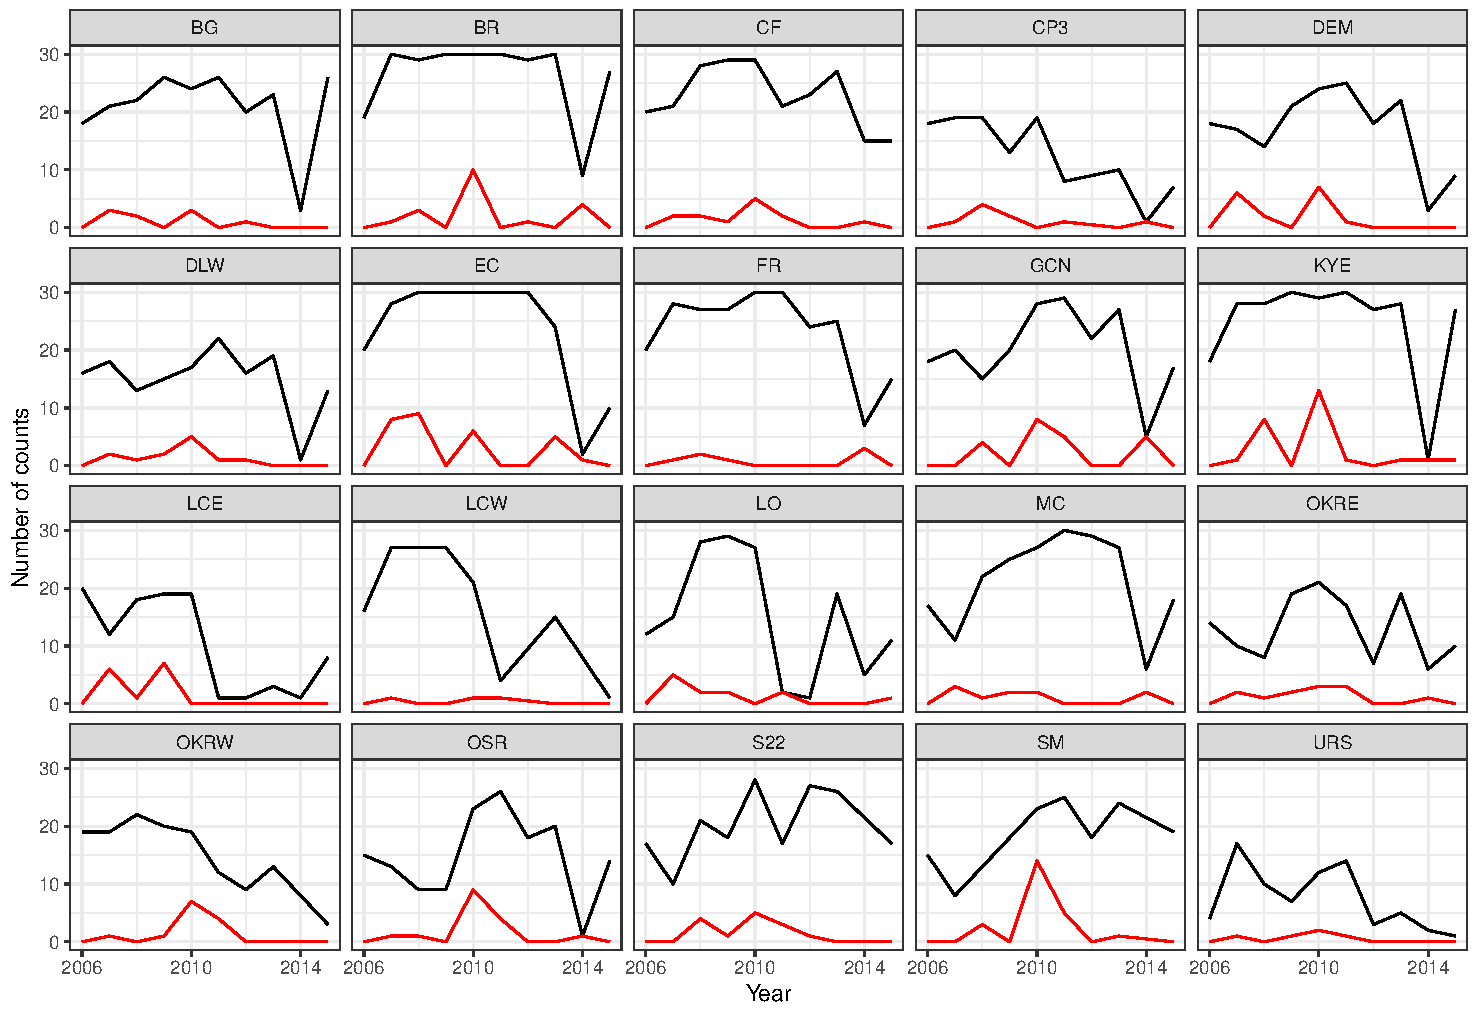
\includegraphics[width=\textwidth]{/Users/gregor/Dropbox/clarkiaSeedBanks/products/figures/underCounting.pdf}  
    \caption{ Graphical summary of undercounting in the dataset on seedling survival to fruiting. Each panel summarizes the datasets on seedling survival to fruiting (Tables~\ref{tab:sigma} and~\ref{tab:undercount}). The black lines correspond to total plots with data on seedling survival. The red lines correspond to the number of plots with fewer seedlings than fruiting plants in a plot (corresponding to undercounting). }
 \label{fig:obs_pred}
\end{figure}
 
  \newpage
 
%%%%%%%%%%%%%%%%%%%%%%%%%%%%%%%%%%
% FRUITS PER PLANT
%%%%%%%%%%%%%%%%%%%%%%%%%%%%%%%%%%

...

  \newpage
 
%%%%%%%%%%%%%%%%%%%%%%%%%%%%%%%%%%
% SEEDS PER FRUIT
%%%%%%%%%%%%%%%%%%%%%%%%%%%%%%%%%%
 
 % latex table generated in R 3.6.2 by xtable 1.8-4 package
% Wed Mar 25 10:18:59 2020
\captionof{table}{ Summary of dataset on seeds per undamaged fruit. [Data set $\bm{\mathrm{Y}}_8$] } \label{tab:titleviab} 
\begin{table}[ht]
\centering
\begin{tabular}{lcccccccccc}
  \hline
  \hline
Population & 2006 & 2007 & 2008 & 2009 & 2010 & 2011 & 2012 & 2013 & 2014 & 2015 \\ 
  \hline
BG &  21 &  21 &  41 &  30 &  30 &  28 &   1 &  29 &  30 &  29 \\ 
  BR &  20 &  20 &  32 &  30 &  29 &  18 &   1 &  29 &  31 &  31 \\ 
  CF &  20 &  20 &  30 &  29 &  34 &  30 &   3 &  27 &  30 &  26 \\ 
  CP3 &  20 &  20 &  41 &  30 &  30 &  29 &   9 &  21 &  30 &  21 \\ 
  DEM &  20 &  20 &  29 &  30 &  32 &  27 &   3 &  27 &  24 &  28 \\ 
  DLW &  20 &  20 &  22 &  30 &  31 &  28 &   5 &  25 &   1 &  30 \\ 
  EC &  20 &  20 &  29 &  30 &  31 &  26 &   8 &  22 &  31 &  31 \\ 
  FR &  20 &  20 &  31 &  30 &  31 &  31 &  20 &  10 &  46 &  30 \\ 
  GCN &  20 &  20 &  29 &  30 &  32 &  30 &   1 &  29 &  28 &  29 \\ 
  KYE &  20 &  20 &  30 &  30 &  30 &  30 &   2 &  28 &  30 &  29 \\ 
  LCE &  20 &  20 &  30 &  30 &  32 &  12 & NA & NA &  30 &  38 \\ 
  LCW &  20 &  20 &  28 &  30 &  35 &  32 &  26 &   4 &   1 & NA \\ 
  LO &  32 &  32 &  30 &  30 &  37 &   2 &  28 &   2 &  30 & NA \\ 
  MC &  20 &  20 &  29 &  30 &  35 &  30 &   4 &  26 &  46 &  35 \\ 
  OKRE &  20 &  20 &  26 &  30 &  30 &  28 &  27 &   3 &  18 &  24 \\ 
  OKRW &  20 &  20 &  33 &  30 &  34 &  28 &  26 &   4 &   9 & NA \\ 
  OSR &  20 &  20 &  32 &  30 &  30 &  28 &   1 &  29 &  30 &  37 \\ 
  S22 &  20 &  20 &  33 &  30 &  28 &  23 & NA &  30 &  23 &  30 \\ 
  SM &  20 &  20 &  31 &  29 &  32 &  30 &   3 &  27 &   3 &   8 \\ 
  URS &  18 &  30 &  25 &  30 &  30 &  27 &  25 &   5 &   1 & NA \\ 
   \hline
\end{tabular}
\end{table}
 
\end{document}